%This is a LaTeX file for producing Adobe portable
%document files suitable for AMS extended abstracts.
%	Christopher M. Godfrey
%	University of North Carolina Asheville
%
%%%%%%%%%%%%%%%%%%%%%%%%%%%%%%%%%%%%%%%%%%%%%%%%%%
\documentclass[twocolumn]{article}

\usepackage{preprint}	%Use style file 'preprint.sty'
\usepackage{epsfig}		%Use postscript (.eps figures)
\usepackage{indentfirst}%Indent the first paragraph in each section
\usepackage{graphicx}	%Allows \includegraphics
\usepackage{epic}		%Allows picture
\usepackage{eepic} 		%Allows more commands to work in picture
\usepackage{float} 		%Allows use of [H] option on floats
\usepackage{textcomp}	%Makes special symbols where necessary (need 'textcomp.sty')
\usepackage{amsmath}	%Adjusts size of delimiters in equations

%Use this if you're brave and want multiple columns - beware of float problems!
%\usepackage{multicol}

\graphicspath{{./figures/}}	%Store figures separately

%Change the way figures are labeled
\renewcommand{\figurename}{\textsc{Fig.}}

%Change the way tables are labeled
\renewcommand{\tablename}{\textsc{Table}}

%Change the font in captions to make text smaller
\newcommand{\captionfonts}{\footnotesize}

%Modify caption styles to match AMS format
\makeatletter  % Allow the use of @ in command names
\long\def\@makecaption#1#2{%
  %\vskip\abovecaptionskip	%Adds extra space below a figure/before a caption
  \sbox\@tempboxa{{\captionfonts #1. #2}}%
  \ifdim \wd\@tempboxa >\hsize
    {\captionfonts #1. #2\par}
  \else
    \hbox to\hsize{\hfil\box\@tempboxa\hfil}%
  \fi
  \vskip\belowcaptionskip}
\makeatother   % Cancel the effect of \makeatletter

%Fix floats in multicolumn environment - also works with 'twocolumn' class
\makeatletter
\newenvironment{tablehere}
  {\def\@captype{table}}
  {}
\newenvironment{figurehere}
  {\def\@captype{figure}}
  {}
\makeatother

%Uncomment to center the last line of captions
%\usepackage{ccaption}
%\captionstyle{\centerlastline}

%%%%%%%%%%%%%%%%%%%%%%%%%%%%%%%%%%%%%%%%%%%%%%%%%%
%Start article here
\begin{document}

%Span both columns
\twocolumn[%

%Insert small space at top of title page
\vspace{0.125in}

%Insert the paper number
{\textbf{
%%%My paper number is...>>>>>>>>>>
JP1.2
%%%<<<<<<<<<<<<<<<<<<<<<<<<<<<<<<<
}}

%Bring the title back up to the same line as the paper number
%%%>>>>>>>>>>UNCOMMENT ONE>>>>>>>>
%\vspace{-0.39in}	%My title is large
\vspace{-0.354in}	%My title is small
%%%<<<<<<<<<<<<<<<<<<<<<<<<<<<<<<<

%Make the title
\begin{center}
\setstretch{1.3}	%Sets title line spacing

%%%>>>>>>>>>>UNCOMMENT ONE>>>>>>>>
%{\textbf{\large{	%My title is large/bold
%{{\large{			%My title is large/not bold
{\textbf{{			%My title is small/bold
%{{{				%My title is small/not bold
%%%Title>>>>>>>>>>>>>>>>
SOIL TEMPERATURE AND MOISTURE ERRORS IN ETA MODEL ANALYSES
%%%<<<<<<<<<<<<<<<<<<<<<
}}}
\end{center}
\begin{center}
%%%First Author>>>>>>>>>>>>>>>
Christopher M. Godfrey$^{*}$
%%%<<<<<<<<<<<<<<<<<<<<<
\\
%%%Affiliation>>>>>>>>>>
University of Oklahoma, Norman, Oklahoma\\
%%%<<<<<<<<<<<<<<<<<<<<<

%%%Second Author>>>>>>>>>>>>>>>
{\hspace{0.01in}}\\
David J. Stensrud
%%%<<<<<<<<<<<<<<<<<<<<<
\\
%%%Affiliation>>>>>>>>>>
NOAA/National Severe Storms Laboratory, Norman, Oklahoma\\
%%%<<<<<<<<<<<<<<<<<<<<<

%%%Third Author>>>>>>>>>>>>>>>
{\hspace{0.01in}}\\
Lance M. Leslie
%%%<<<<<<<<<<<<<<<<<<<<<
\\	%Don't forget to uncomment this line
%%%Affiliation>>>>>>>>>>
University of Oklahoma, Norman, Oklahoma\\
%%%<<<<<<<<<<<<<<<<<<<<<
\vspace{3mm}
\end{center}

]	%You need this bracket!

%Create the corresponding author footnote
{\textfloatsep 0.1875in
\begin{table}[!b]
\hrule height 0.05pt width 0.5625in	%Horizontal line
\vspace{0.125in}
\setstretch{0.76}	%Adjust line spacing
{\footnotesize
%\hspace{2mm}		%No indent for preprints
{\it $^{*}$Corresponding author address:}
%>>>>>>>>>PLACE CORRESPONDING AUTHOR HERE>>>>>>>>>>>>>>>
Christopher M. Godfrey, University of Oklahoma, School of Meteorology, 
100 E. Boyd Street, Suite 1310, Norman, Oklahoma 73019; e-mail: christopher.godfrey@noaa.gov.
%<<<<<<<<<<<<<<<<<<<<<<<<<<<<<<<<<<<<<<<<<<<<<<<<<<<<<<<
%Use "\\" above to break the line between postal and email addresses (non-preprint)
}
\end{table}
}

%PLACE TEXT OF ARTICLE HERE>>>>
\section{{\normalsize \hspace{-0.195in} {\textbf{
%%%Insert section heading below>>>>>>>>>>>>
INTRODUCTION
%%%<<<<<<<<<<<<<<<<<<<<<<<<<<<<<<<<<<<<<<<<
}}}} \vspace{-1.6mm}
\label{etacomp_intro.sec}
Numerical weather prediction models require an accurate representation of initial land surface conditions in order to partition properly the sensible and latent heat fluxes that drive the evolution of the planetary boundary layer.  Models accomplish this exchange of energy between the land surface and the atmosphere through land surface parameterizations (e.g., Bhumralkar 1975; Blackadar 1976; Deardorff 1978; McCumber and Pielke 1981; Pan and Mahrt 1987; Noilhan and Planton 1989), in which the ground heat flux plays a critical role in the surface energy balance.  The ground heat flux in turn depends heavily upon soil temperature and soil moisture conditions, as well as vegetation coverage, atmospheric conditions, and the physical properties of the soil.  Soil moisture provides a key link between the atmosphere and the water and energy balances at the surface of the earth (Wei 1995; Robock et al. 2000; Leese et al. 2001).  It influences the available water for plant transpiration, and plays a role in the mass balance for many forecast models.  Soil thermal conductivity estimates, which facilitate the proper heat transfer within the soil, also strongly depend upon soil moisture specifications.  To calculate soil heat transfer, the most sophisticated land surface parameterizations require not only near-surface soil temperatures, but also temperature profiles (e.g., Viterbo and Beljaars 1995; Chen and Dudhia 2001).  Together, soil temperature and moisture work in concert to directly influence ground, sensible, and latent heat fluxes and affect forecasts of temperature, mixing ratio, precipitation, and cloud cover.

Several studies have demonstrated sensitivities of forecasts of near-surface variables to soil water content.  An inspection of the relationship between soil moisture variations and surface turbulent energy fluxes for a variety of vegetation types reveals that energy fluxes display more sensitivity for dry soils than for wet soils and that sparsely vegetated areas require more accurate soil moisture observations or simulations (Dirmeyer et al. 2000).  Changes in soil moisture modify the balance between latent and sensible heat fluxes and can influence surface temperatures or affect turbulent transfer in the boundary layer (McCumber and Pielke 1981).  For example, Pan and Mahrt (1987) couple a one-dimensional model of the planetary boundary layer (Troen and Mahrt 1986) with a two-layer soil hydrology model (Mahrt and Pan 1984) and find that surface evaporation can drive boundary-layer development.

Soil moisture also influences the development of deep convection due to the influence of soil moisture on latent heat fluxes and boundary layer moisture (Clark and Arritt 1995).  Yan and Anthes (1988) investigate the effect of soil moisture variations on precipitation patterns by simulating adjacent strips of moist and dry land.  They find that for sufficiently wide horizontal strips under convectively unstable conditions, the inhomogeneities in surface moisture lead to gradients of ground temperature that eventually help produce sea-breeze circulations and an increase in convective rainfall.  This result compliments the observations of Pielke and Zeng (1989), who show increases in available buoyant energy when irrigated land lies adjacent to natural grassland, compared with natural grassland alone.  Soil moisture further affects boundary-layer cloud development by increasing cloud cover for both moist and dry soils, depending on the strength of the stability above the boundary layer (Ek and Holtslag 2004).

Numerical and observational studies of soil moisture reveal that soil moisture anomalies influence regional atmospheric conditions over time scales of two to three months (Liu et al. 1993; Vinnikov et al. 1996), with variations in temporal scales of soil moisture attributable to the seasonal cycle of potential evaporation (Entin et al. 2000).  After simulating soil moisture anomalies, there is evidence that soil moisture affects model forecasts of precipitation, atmospheric moisture, and temperature for several weeks (Walker and Rowntree 1977; Rowntree and Bolton 1983).  Modeling studies of soil temperature and moisture conditions show that differing soil moisture initializations influence monthly or seasonal temperatures and precipitation patterns (Rind 1982; Betts et al. 1996) and that these initial conditions again possess a persistence time scale of months to seasons (Yeh et al. 1984; Walsh et al. 1985; Vinnikov and Yeserkepova 1991; Gao et al. 1996; Liu and Avissar 1999a,b).  Monthly forecasts also show sensitivity to initial soil moisture conditions, displaying increased skill for precipitation and air temperature forecasts with more realistic land surface initializations (Koster et al. 2004).  Other studies report that soil moisture anomalies also affect extreme precipitation forecasts on monthly time scales (Beljaars et al. 1996; Viterbo and Betts 1999).  In seasonal predictions, Fennessy and Shukla (1999) investigate the role of initial soil moisture using ensembles of global climate model simulations and find that increases in initial soil wetness lead to increased seasonal evaporation, decreased seasonal mean surface air temperatures, and generally increased seasonal mean precipitation in many regions.  Other authors assert that the seasonal evolution of the atmosphere in a regional atmospheric model is dependent upon initial soil moisture and landscape specification (Pielke et al. 1999).  Thus, when compared with soil temperature, soil moisture clearly has more interannual variability and more strongly influences forecasts (Liu and Avissar 1999a,b; Rodell et al. 2005).

While soil moisture appears to be the most important factor for land-surface initializations (Gannon 1978; McCumber and Pielke 1981; Smith et al. 1994), one should not underestimate the role of soil temperature in the evolution of the lower atmosphere, especially for short-range forecasts.  Longwave radiation loss is a function of soil temperature and directly affects the radiation budget at the surface.  Ground heat flux also is a function of soil temperature (Brotzge and Crawford 2003), and affects the sensible heat flux, boundary layer growth and decay, turbulence, and air temperature.  Clearly, forecast models require both accurate soil temperature and soil moisture initializations.  Though efforts are under way to provide more extensive networks of soil moisture data from a variety of remote sensing and direct observational sources (Entekhabi et al. 1999; Leese et al. 2001; Seuffert et al. 2004), routine \textit{in situ} observations of soil temperature and moisture suitable for data assimilation are currently unavailable over large areas of the continental United States and the world.

Due to the absence of a large observational soil-monitoring network, many forecast models implement complex land surface models to realistically determine soil hydrology.  The National Centers for Environmental Prediction (NCEP) operational Eta model (Black 1994) produces land surface analyses by continuously cycling temperature and moisture fields within the Noah land surface model (LSM, Chen et al. 1996; Koren et al. 1999).  In the past, these fields evolved only in response to radiation budget constraints and modeled precipitation, but NCEP recently upgraded the self-cycling process so that soil fields respond instead to adjusted precipitation observations from both radar and gauge data over the United States.

Many modeling efforts have used NCEP Eta model analyses and forecasts over the continental United States as initial and boundary conditions for a variety of applications (e.g., Colle et al. 2001; Bright and Mullen 2002; Stensrud and Weiss 2002; Westrick et al. 2002; Zhender 2002; Brennan et al. 2003; Chen et al. 2004; Hart et al. 2004; Hoadley et al. 2004; Galewsky and Sobel 2005; Zamora et al. 2005; Zhong et al. 2005).  The Eta model therefore provides very important initial land-surface conditions that strongly influence forecasts for both operational and research purposes.  Unfortunately, many land surface models, including the Noah LSM, do not capture observed soil moisture variations when forced with atmospheric observations or cycled model output (Robock et al. 2000).  Marshall et al. (2003) found a strong positive bias in soil moisture from the Eta model in comparison to Oklahoma Mesonet observations, but also noted that a change in the Eta model initialization procedure to a continuous self-cycling initialization for soil moisture significantly mitigated this bias.  Marshall et al. (2003) also reported a warm bias in soil temperatures at a depth of 5 cm in the late afternoon and a cool bias in the early morning.  On the other hand, Robock et al. (2003) found good agreement when comparing soil temperature and moisture output from a more recently implemented version of the Noah LSM with observations from the Oklahoma Mesonet averaged over all of Oklahoma during 1998--99.

This study compares Eta model analyses of soil temperature and moisture at 0000 UTC and 1200 UTC with observations from the Oklahoma Mesonet between 1 March 2004 and 1 October 2005.  In contrast to the findings of Robock et al. (2003), strong biases in soil temperature exist, as well as a severe underestimation of soil moisture at all depths.  An important distinction between this and previous studies is that the results derive from point comparisons, rather than large-scale averages.  The reasoning behind this decision appears in section 4.


\section{{\normalsize \hspace{-0.195in} {\textbf{
%%%Insert section heading below>>>>>>>>>>>>
MODEL DESCRIPTION
%%%<<<<<<<<<<<<<<<<<<<<<<<<<<<<<<<<<<<<<<<<
}}}} \vspace{-1.6mm}
\label{etacomp_desc.sec}
The National Centers for Environmental Prediction (NCEP) Eta model (Black 1994) is initialized from analyses provided by the Eta Data Assimilation System (EDAS, Rogers et al.\ 1996; Nelson 1999).  The EDAS first produces a 3-h forecast from its own analysis over the continental United States. The system then uses this forecast as a background field for assimilating subsequent observations over this 3-h period and produces a new analysis valid at the end of the 3-h window.  This process continues indefinitely, with forecasts out to 84 hours produced from the most recent EDAS analysis every six hours.  The Eta model produces each EDAS forecast so that initial atmospheric and soil conditions are consistent with the forecast model and match its resolution, physics, and dynamics (Rogers et al.\ 1996).  The absence of a complete set of observations of soil temperature and soil moisture necessitates continuously self-cycled soil fields within the EDAS without observational corrections or soil moisture nudging toward climatology.  These soil fields evolve only in response to external forcing from model physics and surface forcing in the form of precipitation and the surface radiation balance within the EDAS.

Prior to a modification on 16 March 2004, the EDAS assimilated hourly precipitation data consisting of radar and gauge observations from NCEP Stage II and Stage IV analyses (Fulton et al.\ 1998; Lin et al.\ 2005). These analyses exhibit a systematic dry bias which, when used as the driver for soil moisture, leads to drier soil.  After an adjustment on this date, comparisons of the cumulative 24-h precipitation from EDAS against daily gauge analyses, inflated by 10\% to correct for catchment errors, yield a long history of net deficits or surpluses in precipitation.  Adjustments to the EDAS hourly precipitation input based on this history attempt to eliminate the deficit or surplus over 24 hours.  Adjustments remain limited to $\pm$ 20\% of the hourly precipitation analysis values and only apply to grid points in the analysis with non-zero precipitation.  The EDAS assimilates the adjusted hourly precipitation input and then models the precipitation field.  This modeled precipitation drives the land surface physics, though the modeled precipitation does not necessarily match the bias-adjusted observations (Lin et al.\ 2005).  

A more extensive modification to the land surface scheme occurred on 3 May 2005 in the operational Eta model, now termed the North American Mesoscale (NAM).  Previously, the EDAS would create precipitation during the assimilation process in regions where the Eta model did not forecast precipitation.  The renamed NAM Data Assimilation System (NDAS) no longer adjusts precipitation totals in locations where the precipitation from the NAM model is less than the bias-adjusted observations.  However, the latent heat and moisture fields are reduced where the modeled precipitation is greater than the bias-adjusted observations.  More importantly, the NDAS drives the land surface physics directly with the bias-adjusted observations rather than with the NDAS modeled precipitation, resulting in moister soil.  The previous version tended toward a dry bias during the assimilation because the modeled precipitation did not exactly replicate observed precipitation coverage and intensities.  This allows for a more robust and more accurate precipitation assimilation that increases soil moisture.  Additionally, there is no longer an upper limit for cloud water mixing ratios when computing optical depths, which improves radiation absorption, and modifications to the cloud cover parameterization allow for more fractional cloudiness (DiMego and Rogers 2005).

Simultaneous upgrades to the Noah LSM addressed low-level temperature and humidity biases.  Vegetation and soil databases have more classes with higher spatial resolution.  A 1-km resolution, United States Geological Survey (USGS) 24-class vegetation type database replaced the 13-class, 1-degree resolution simple biosphere (SiB) vegetation types (Sellers et al. 1986).  For soil characteristics, the 1-km resolution, 16-class State Soil Geographic Database (STATSGO, Miller and White 1998) data eclipsed the 1-km resolution, nine-class Zobler soil types (Zobler 1986).  A 1-degree database of soil temperatures at the lower boundary at 300 cm depth replaced an old 2.5-degree soil temperature database.  In addition, model developers lowered the leaf area index and compensated for the effect of the new precipitation assimilation procedures on the existing soil moisture bias by tuning the canopy conductance and other vegetation parameters within the Noah LSM.  A lowered roughness length for heat reduces the skin temperature, thereby lowering the 2-m temperature forecasts and reducing the warm bias, though this does not change latent or sensible heat fluxes significantly.  Overall, these modifications reduce drying trends and increase the low-level moisture (DiMego and Rogers 2005).

\section{{\normalsize \hspace{-0.195in} {\textbf{
%%%Insert section heading below>>>>>>>>>>>>
DATA
%%%<<<<<<<<<<<<<<<<<<<<<<<<<<<<<<<<<<<<<<<<
}}}} \vspace{-1.6mm}
\label{etacomp_data.sec}
The Oklahoma Mesonet is an integrated network of 116 automated surface observing stations, with at least one site in each of Oklahoma's seventy-seven counties.  Each site measures atmospheric variables every five minutes and soil temperature at a depth of 10 cm every 15 minutes under both bare soil and native vegetation.  Most of the sites also measure soil temperature at a depth of 5 cm under both bare soil and native vegetation and at a depth of 30 cm under native vegetation.  Many Oklahoma Mesonet sites also report soil moisture at depths of 5, 25, 60, and 75 cm.  All data fall subject to rigorous quality assurance procedures to ensure the production of reliable, research-quality data (Shafer et al. 2000).  A complete description of the Oklahoma Mesonet, including sensor specifications, appears in Brock et al. (1995), while Basara and Crawford (2000) discuss the soil moisture instrumentation.

\section{{\normalsize \hspace{-0.195in} {\textbf{
%%%Insert section heading below>>>>>>>>>>>>
COMPARISON WITH OBSERVATIONS
%%%<<<<<<<<<<<<<<<<<<<<<<<<<<<<<<<<<<<<<<<<
}}}} \vspace{-1.6mm}
\label{etacomp_comp.sec}
Gridded 40-km Eta model analyses of soil temperature and moisture at 0000 UTC and 1200 UTC were bilinearly interpolated to Oklahoma Mesonet observation sites allowing for direct model verification.  While Eta model soil analyses are available at the present operational grid spacing of 12 km, researchers seldom use these analyses for initializing forecast models.  Comparisons span the period from 1 March 2004 through 1 October 2005.  This period is sufficient to characterize the performance of the EDAS soil temperature and moisture schemes both before and after the change from continuously self-cycling modeled precipitation and radiation to assimilation of precipitation observations on 3 May 2005.

Point measurements of soil temperature and moisture are not as spatially representative as atmospheric measurements, primarily due to spatial heterogeneities in vegetation coverage and soil types (Marshall et al. 2003; Brotzge and Crawford 2003).  For this reason, spatial and temporal averaging of observations reduces small-scale noise and enables model validation and intercomparisons (e.g., Marshall et al. 2003; Robock et al. 2003).  However, interpolating observations to a model grid yields comparisons that are partly a function of the interpolation scheme rather than the underlying observations.  An analysis scheme cannot account for small spatial variations in the observations and thus analyzed and observed values may differ considerably (Schlatter 1975).  Moreover, individual observation points, and not areal averages, provide the raw data for objective analysis schemes that produce gridded initial conditions for models.  It is therefore important to correctly estimate point values of soil temperature and soil moisture in the Eta model so that these values can provide meaningful initial conditions for other numerical models with different grid sizes.  The choice to analyze point comparisons in this study rather than interpolate the observations to the model grid permits a bulk characterization of the model performance over all of Oklahoma without introducing errors through large-scale spatial averaging.
%%%%%%%%%%%%%%%%%%%%%%%%%%%%%%%%%%%%%%%%%%%%%%%%%%%%%%%%%%%%%%%%%%%%
\begin{figure}[!t] %[!htbp]
\begin{center}
\includegraphics[angle=0, width=0.48\textwidth]{etacompfig1col}
\end{center}
\caption{
Soil temperature (K) at 0000 UTC 15 July 2005 from a) Oklahoma Mesonet observations
at a depth of 5-cm under sod and b) the 0--10 cm soil layer of the 0000 UTC Eta
analysis.
\label{etacompfig1}
}
\end{figure}
%%%%%%%%%%%%%%%%%%%%%%%%%%%%%%%%%%%%%%%%%%%%%%%%%%%%%%%%%%%%%%%%%%%%

Though comparisons between the Eta model and observations only include point measurements, Figures~\ref{etacompfig1} and~\ref{etacompfig2} provide informative visualizations of the geographic variability of Oklahoma Mesonet 5-cm soil temperature and moisture observations compared with Eta model 0--10 cm soil temperature and moisture analyses for a representative summer day.  The Oklahoma Mesonet observations are interpolated to a 3-km horizontal grid using a two-pass Barnes analysis (Barnes 1973).  The Eta analyses, shown here interpolated to the same 3-km horizontal grid, display a cool and dry bias typical of many 1200 UTC analyses.  In addition, the differences in the patterns of each field can influence the subsequent forecast.
%%%%%%%%%%%%%%%%%%%%%%%%%%%%%%%%%%%%%%%%%%%%%%%%%%%%%%%%%%%%%%%%%%%%
\begin{figure}[!t] %[!htbp]
\begin{center}
\includegraphics[angle=0, width=0.48\textwidth]{etacompfig2col}
\end{center}
\caption{
Soil moisture (m$^3$ m$^{-3}$) at 0000 UTC 15 July 2005 from a) Oklahoma Mesonet observations
at a depth of 5-cm and b) the 0--10 cm soil layer of the 0000 UTC Eta
analysis.
\label{etacompfig2}
}
\end{figure}
%%%%%%%%%%%%%%%%%%%%%%%%%%%%%%%%%%%%%%%%%%%%%%%%%%%%%%%%%%%%%%%%%%%%

The Noah LSM model within the EDAS contains five soil layers representing depths of 0--10 cm, 10--40 cm, 40--100 cm, and 100--200 cm, and a constant reservoir temperature at 300 cm.  Soil temperatures in the 0--10 cm model layer are compared with Oklahoma Mesonet observations at a depth of 5 cm and soil temperatures in the 10--40 cm model layer are compared with observations at a depth of 30 cm.  For soil moisture, the values from the Eta analysis in the 0--10 cm, 10--40 cm, and 40--100 cm layers are compared with observations at depths of 5 cm, 25 cm, and 60 cm, respectively.  These direct comparisons allow computation of root-mean-square error (rmse) and bias (Wilks 1995) across the entire Oklahoma Mesonet.

\subsection{\hspace{-0.09in}{\textit{\textbf{
%Enter subsection heading here:
Soil temperature
}}}}
\label{etacomp_temp.sub}
%%%%%%%%%%%%%%%%%%%%%%%%%%%%%%%%%%%%%%%%%%%%%%%%%%%%%%%%%%%%%%%%%%%%
\begin{figure}[!t] %[!htbp]
\begin{center}
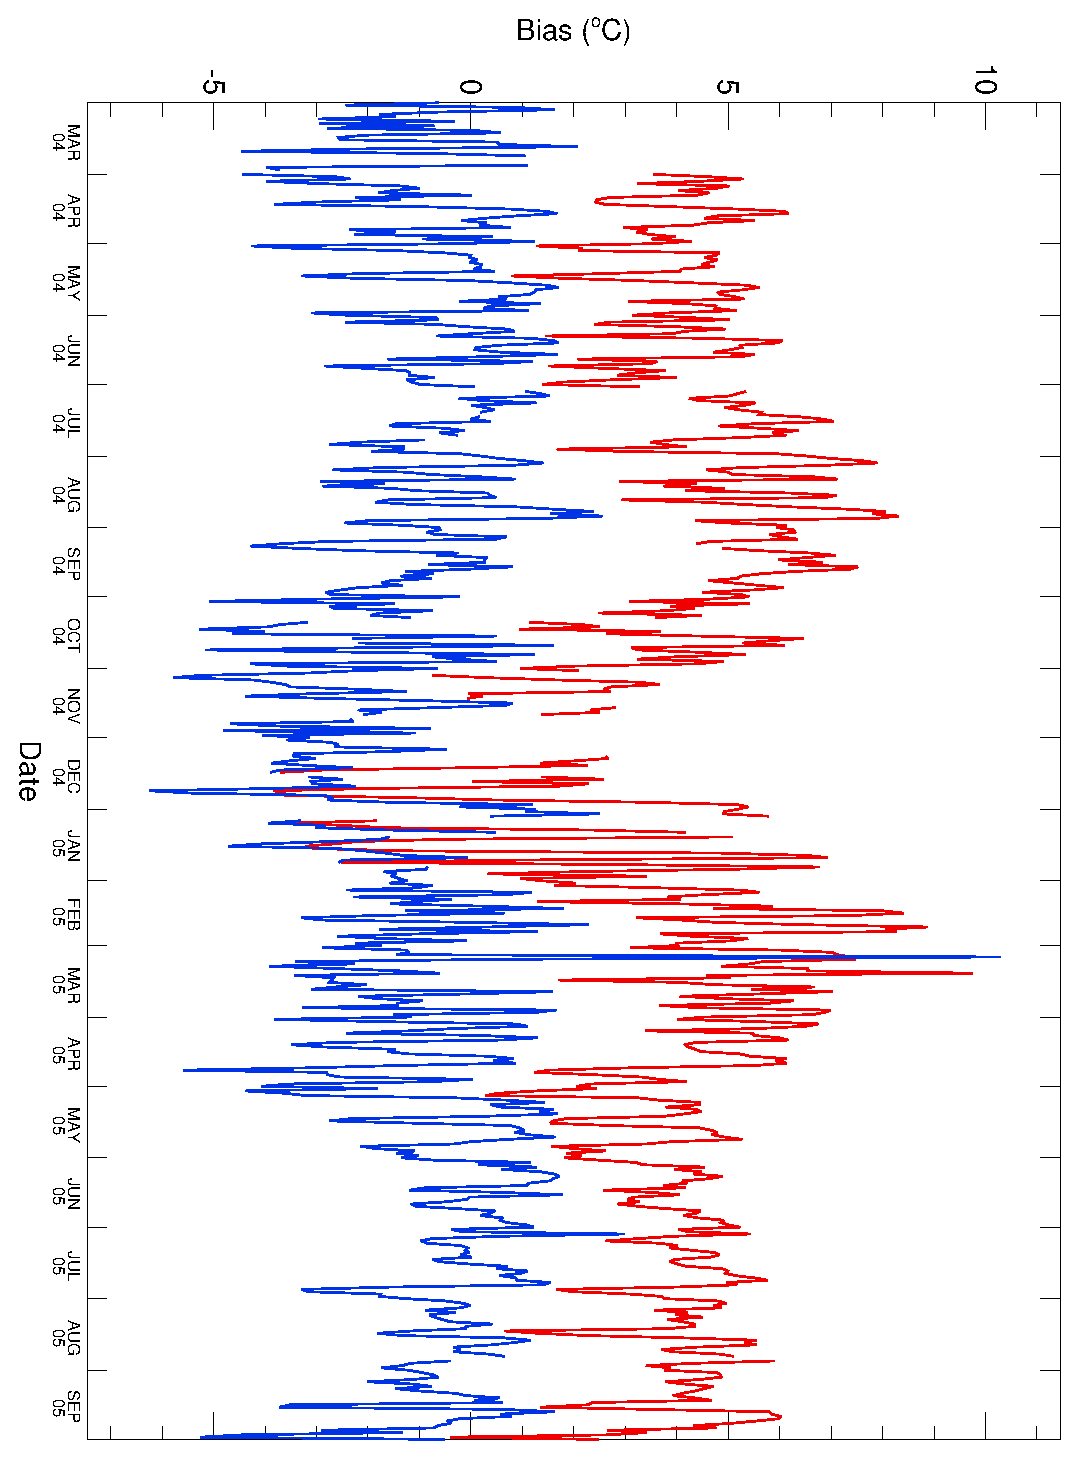
\includegraphics[angle=90, width=0.48\textwidth]{etacompfig3col}
\end{center}
\caption{
Point calculations of daily soil temperature bias (\textdegree{}C) averaged over all of Oklahoma in the 0--10 cm layer
from 0000 UTC (red) and 1200 UTC (blue) Eta analyses compared with 5-cm
soil temperature observations from the Oklahoma Mesonet.
\label{etacompfig3}
}
\end{figure}
%%%%%%%%%%%%%%%%%%%%%%%%%%%%%%%%%%%%%%%%%%%%%%%%%%%%%%%%%%%%%%%%%%%%
%%%%%%%%%%%%%%%%%%%%%%%%%%%%%%%%%%%%%%%%%%%%%%%%%%%%%%%%%%%%%%%%%%%%
\begin{figure}[!t] %[!htbp]
\begin{center}
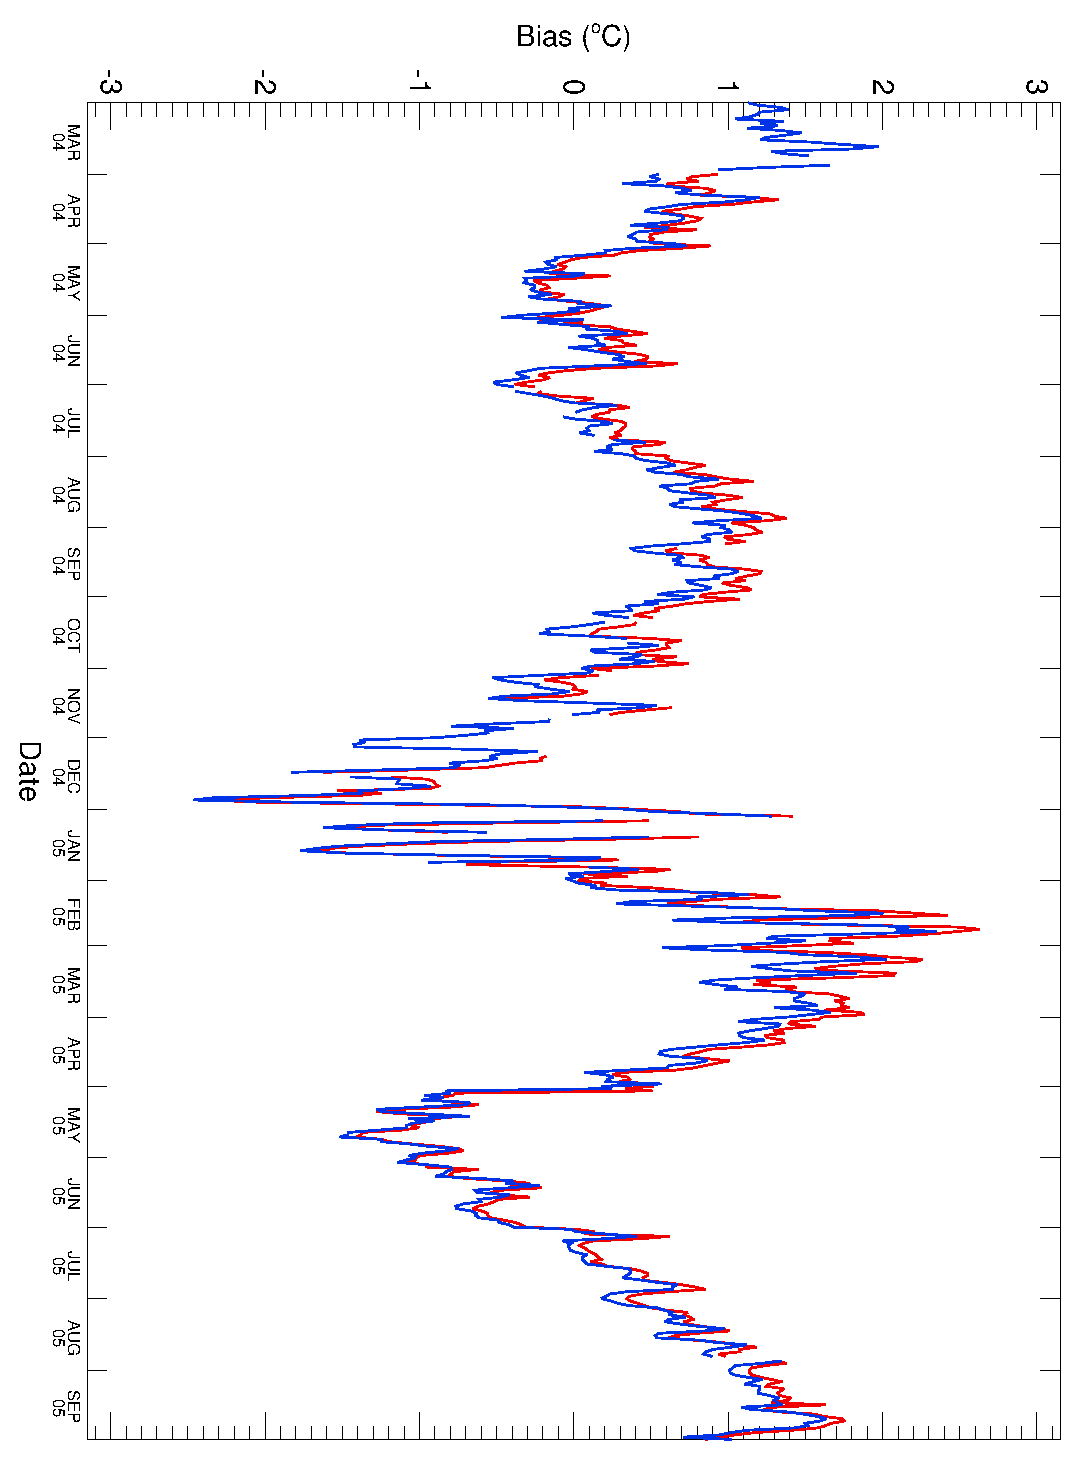
\includegraphics[angle=90, width=0.48\textwidth]{etacompfig4col}
\end{center}
\caption{
Point calculations of daily soil temperature bias (\textdegree{}C) averaged over all of Oklahoma in the 10--40 cm layer
from 0000 UTC (red) and 1200 UTC (blue) Eta analyses compared with 30-cm
soil temperature observations from the Oklahoma Mesonet.
\label{etacompfig4}
}
\end{figure}
%%%%%%%%%%%%%%%%%%%%%%%%%%%%%%%%%%%%%%%%%%%%%%%%%%%%%%%%%%%%%%%%%%%%
There is a strong positive soil temperature bias in the 0--10 cm layer from 0000 UTC Eta model analyses compared with observations of 5-cm soil temperatures from all Oklahoma Mesonet sites (Fig.~\ref{etacompfig3}).  Twelve hours later at 1200 UTC, there is a predominately negative bias.  Overall, the bias for this most shallow soil layer is 4.1{\textdegree}C (-1.0{\textdegree}C) and the rmse is 5.0{\textdegree}C (2.4{\textdegree}C) for 0000 UTC (1200 UTC) Eta analyses.  Errors appear reduced in magnitude in the deeper 10--40 cm soil layer, and the 0000 UTC and 1200 UTC soil temperature analyses differ only slightly (Fig.~\ref{etacompfig4}).  There is a temporally coherent pattern of errors throughout the year such that errors of the same sign persist for multi-week periods.  This trend appears to follow the more variable pattern of daily biases in the upper soil layer.  Modifications to the land surface model on 3 May 2005 do not appear to affect significantly the magnitude of subsequent soil temperature errors.
%%%%%%%%%%%%%%%%%%%%%%%%%%%%%%%%%%%%%%%%%%%%%%%%%%%%%%%%%%%%%%%%%%%%
\begin{figure}[!t] %[!htbp]
\begin{center}
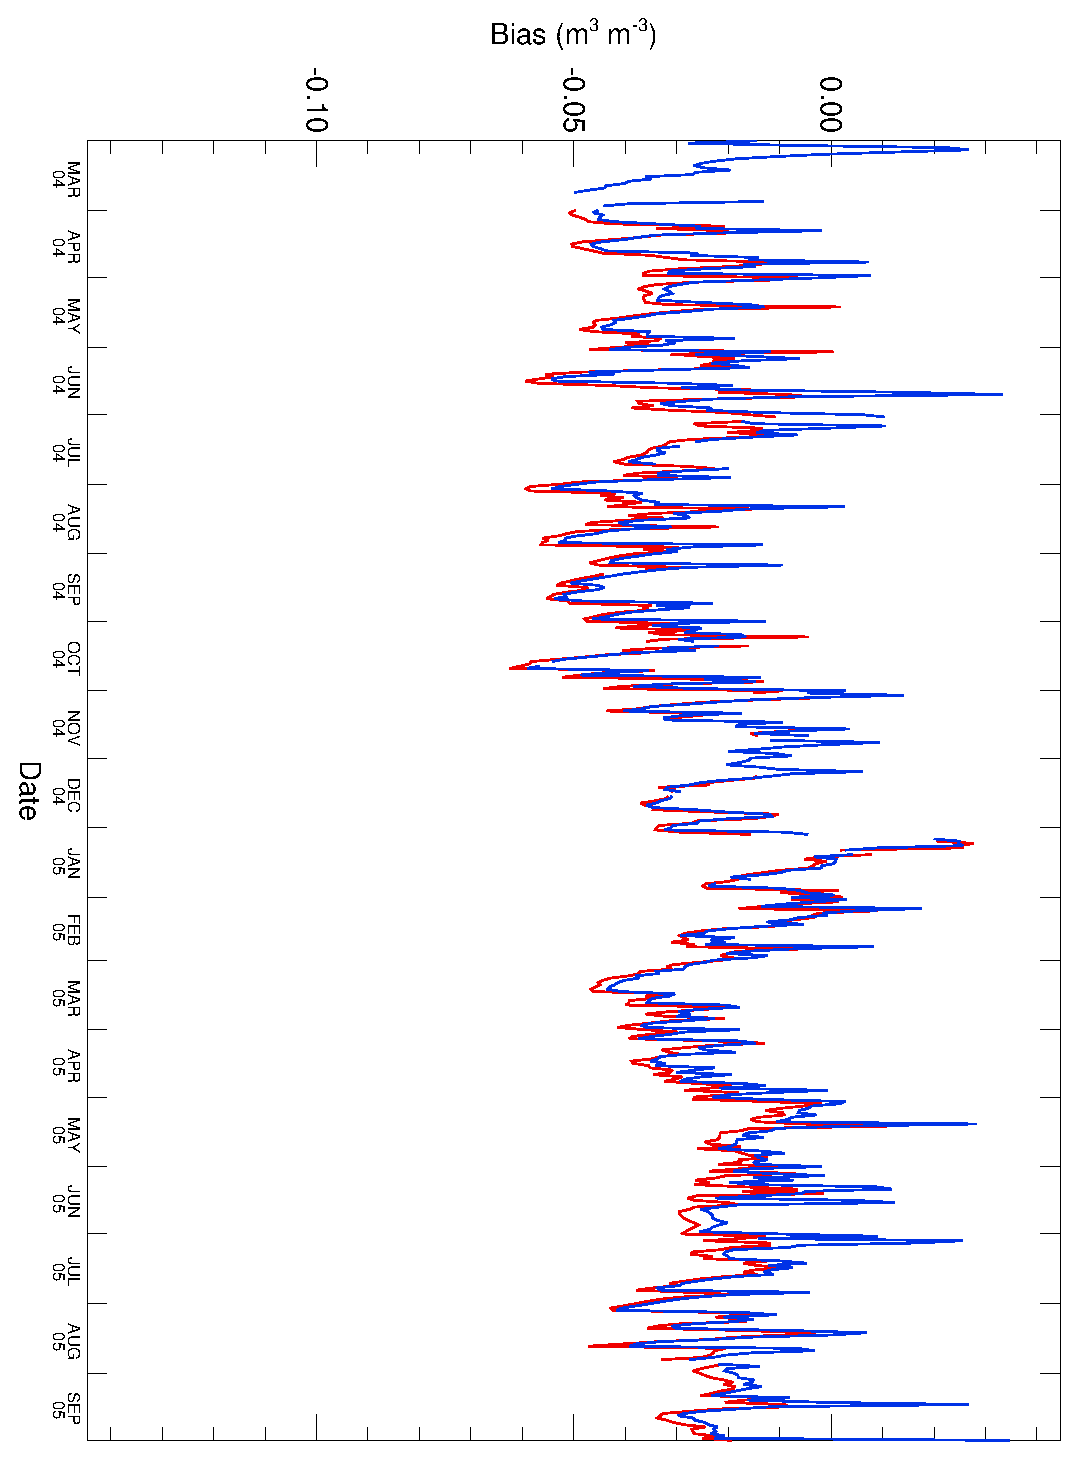
\includegraphics[angle=90, width=0.48\textwidth]{etacompfig5col}
\end{center}
\caption{
Point calculations of daily soil moisture bias (m$^3$ m$^{-3}$) averaged over all of Oklahoma in the 0--10 cm layer
from 0000 UTC (red) and 1200 UTC (blue) Eta analyses compared with 5-cm
soil moisture observations from the Oklahoma Mesonet.
\label{etacompfig5}
}
\end{figure}
%%%%%%%%%%%%%%%%%%%%%%%%%%%%%%%%%%%%%%%%%%%%%%%%%%%%%%%%%%%%%%%%%%%%
%%%%%%%%%%%%%%%%%%%%%%%%%%%%%%%%%%%%%%%%%%%%%%%%%%%%%%%%%%%%%%%%%%%%
\begin{figure}[!t] %[!htbp]
\begin{center}
\includegraphics[angle=90, width=0.48\textwidth]{etacompfig6col}
\end{center}
\caption{
Point calculations of daily soil moisture bias (m$^3$ m$^{-3}$) averaged over all of Oklahoma in the 10--40 cm layer
from 0000 UTC (red) and 1200 UTC (blue) Eta analyses compared with 25-cm
soil moisture observations from the Oklahoma Mesonet.
\label{etacompfig6}
}
\end{figure}
%%%%%%%%%%%%%%%%%%%%%%%%%%%%%%%%%%%%%%%%%%%%%%%%%%%%%%%%%%%%%%%%%%%%

\subsection{\hspace{-0.09in}{\textit{\textbf{
%Enter subsection heading here:
Soil moisture
}}}}
\label{etacomp_moist.sub}
There is a pervasive and persistent dry bias in both the 0000 UTC and 1200 UTC Eta soil moisture analyses.  For each day, the Oklahoma-wide average soil moisture in the 0--10 cm model layer of the Eta analyses is generally drier than the observations at 5 cm (Fig.~\ref{etacompfig5}).  In the 10--40 cm layer, the soil moisture bias slightly exceeds zero for only a single 0000 UTC Eta analysis and in the 40--100 cm layer, the soil moisture bias never becomes positive over the period of study (Figs.~\ref{etacompfig6} and~\ref{etacompfig7}).  Overall, the bias for each soil layer is $-0.03$ m$^3$ m$^{-3}$, $-0.05$ m$^3$ m$^{-3}$, and $-0.09$ m$^3$ m$^{-3}$ for the 0--10 cm, 10--40 cm, and 40--100 cm Eta model layers, respectively.  In the 40--100 cm Eta model layer, the daily average soil moisture error across all of Oklahoma reaches as large as 35\% of the typical range of soil moisture when compared with observations at a depth of 60 cm.

There is notable improvement in the analyzed soil moisture fields after the change from self-cycling precipitation to observed precipitation assimilation on 3 May 2005.  While this change reduced the magnitude of the errors, and evidences itself as a large discontinuity in the bias time series of Figures~\ref{etacompfig6} and~\ref{etacompfig7}, a strong dry bias persists in the soil moisture field.

\section{{\normalsize \hspace{-0.195in} {\textbf{
%%%Insert section heading below>>>>>>>>>>>>
DISCUSSION
%%%<<<<<<<<<<<<<<<<<<<<<<<<<<<<<<<<<<<<<<<<
}}}} \vspace{-1.6mm}
\label{etacomp_disc.sec}
Systematic biases clearly exist in both soil temperature and soil moisture.  Positive soil temperature errors in 0000 UTC Eta analyses likely stem from the documented excess of solar radiation during the daytime (Zamora et al. 2005), while the generally negative soil temperature biases in 1200 UTC Eta analyses result from underestimated downward longwave radiative fluxes during nighttime hours (Stensrud et al. 2005).  Modifications to the land surface physics on 3 May 2005 did not mitigate these errors; soil temperatures in the top soil layer remain too high in the 0000 UTC analyses and dry soil moisture biases continue in each of the top three soil layers.  Tests indicate that these systematic biases in both soil temperature and moisture do not appear to be strongly dependent upon soil or vegetation types defined in Eta model grid cells.

%%%%%%%%%%%%%%%%%%%%%%%%%%%%%%%%%%%%%%%%%%%%%%%%%%%%%%%%%%%%%%%%%%%%
\begin{figure}[!t] %[!htbp]
\begin{center}
\includegraphics[angle=90, width=0.48\textwidth]{etacompfig7col}
\end{center}
\caption{
Point calculations of daily soil moisture bias (m$^3$ m$^{-3}$) averaged over all of Oklahoma in the 40--100 cm layer
from 0000 UTC (red) and 1200 UTC (blue) Eta analyses compared with 60-cm
soil moisture observations from the Oklahoma Mesonet.
\label{etacompfig7}
}
\end{figure}
%%%%%%%%%%%%%%%%%%%%%%%%%%%%%%%%%%%%%%%%%%%%%%%%%%%%%%%%%%%%%%%%%%%%
%%%%%%%%%%%%%%%%%%%%%%%%%%%%%%%%%%%%%%%%%%%%%%%%%%%%%%%%%%%%%%%%%%%%
\begin{figure*}[!t] %[!htbp]
\begin{center}
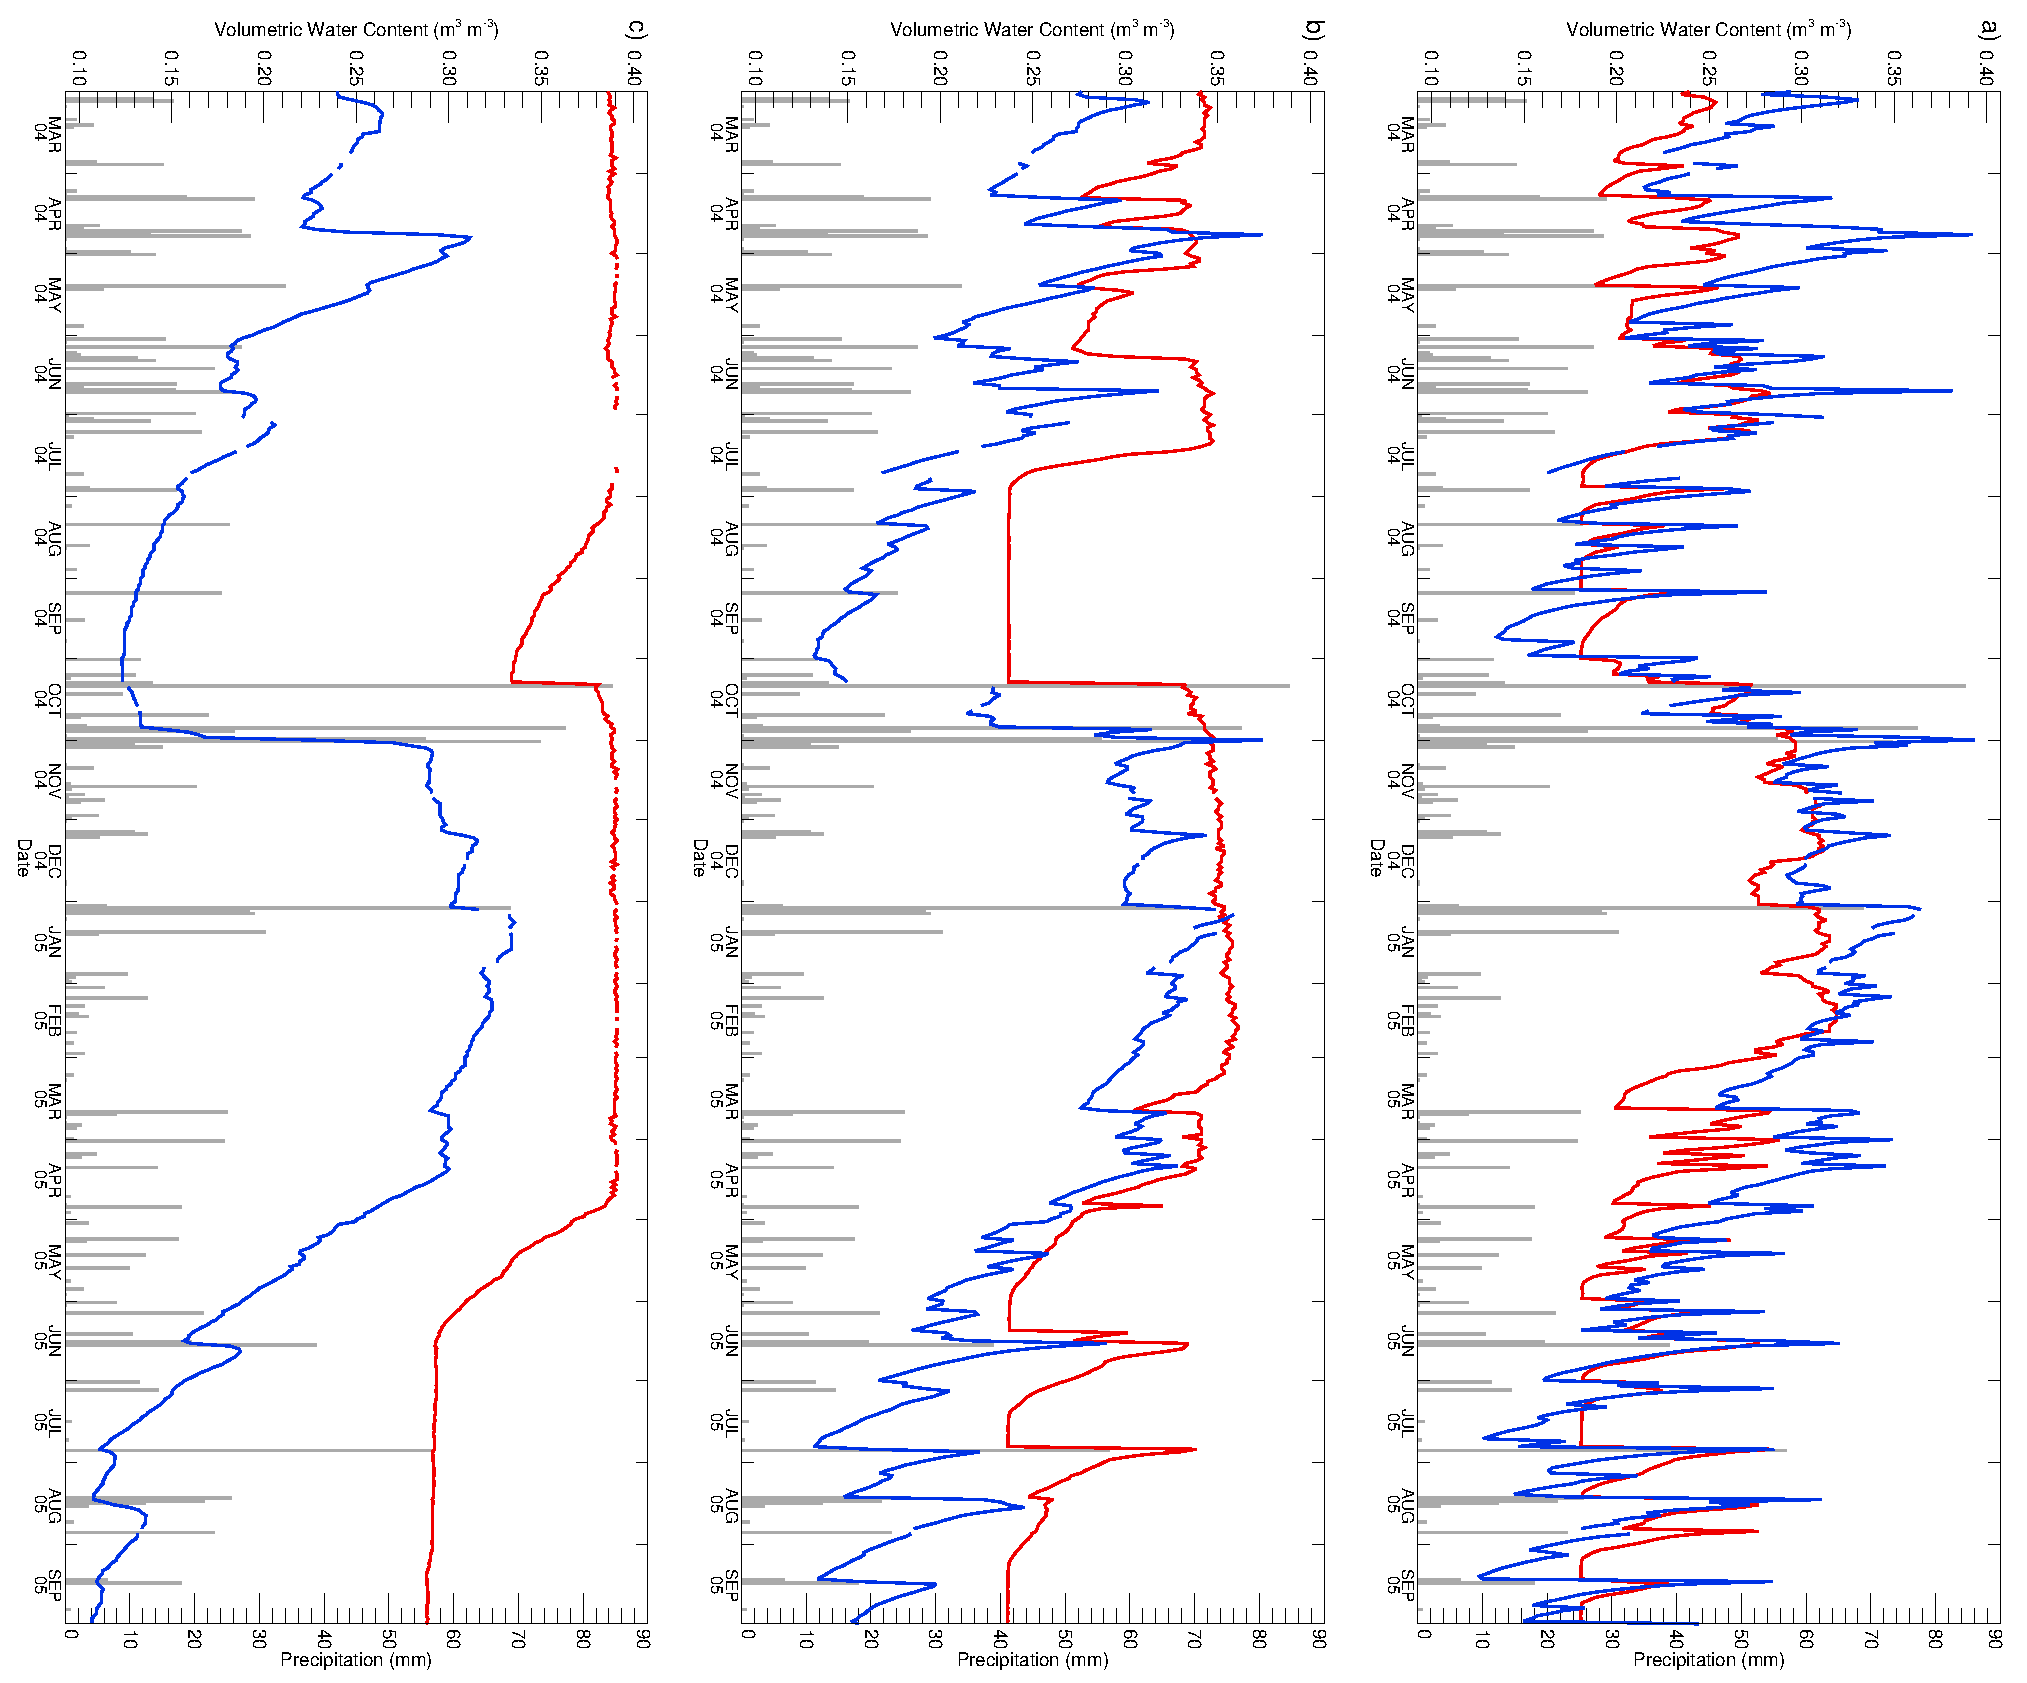
\includegraphics[angle=90, width=0.80\textwidth]{etacompfig8col}
\end{center}
\caption{
Observed soil moisture at 1200 UTC at Eufaula (red) at depths
of a) 5 cm, b) 25 cm, and c) 60 cm compared
with 1200 UTC Eta analyses (blue) in the 0--10, 10--40, and 40--100 cm
soil layers, respectively, and observed daily (0000 UTC--0000 UTC)
precipitation totals (bars).
\label{etacompfig8}
}
\end{figure*}
%%%%%%%%%%%%%%%%%%%%%%%%%%%%%%%%%%%%%%%%%%%%%%%%%%%%%%%%%%%%%%%%%%%%

Figure~\ref{etacompfig8} shows the EDAS soil moisture at three soil depths compared with observed precipitation totals and observed soil moisture at the Eufaula Oklahoma Mesonet site.  The soil moisture errors in the top two model layers result from both an inappropriate response to rainfall events and accelerated desiccation of the soil compared with observations, particularly in the 10--40 cm layer.  The response to precipitation in the 40--100 cm layer appears limited except after several consecutive days of heavy precipitation.  The new precipitation assimilation procedure implemented on 3 May 2005 somewhat improved soil moisture estimates at some Mesonet sites, though systematic dry biases remain in the Eta analyses.

An exploration of the influence of soil heat capacity can help to address the effect of such a dry bias on soil temperatures.  Soil heat capacity is a function of soil moisture and directly affects the diagnosis of soil temperature.  Underestimates of soil moisture such as those in Eta model analyses could therefore result in poorly estimated soil temperatures.  A simple, one-layer slab soil model driven by Oklahoma Mesonet observations allows approximate calculations of the influence of errors in soil moisture alone on soil temperature.  The composite soil volumetric heat capacity employed in the slab model is
%
\begin{equation}\label{etacomp:cg}
C_g=\theta C_{water}+(1-\theta_s)C_{soil}+(\theta_s-\theta)C_{air},
\end{equation}
%
where $\theta$ is the soil volumetric water content, $C_{water} = 4.2 \times 10^6$ J m$^{-3}$ K$^{-1}$, $C_{soil} = 1.26 \times 10^6$ J m$^{-3}$ K$^{-1}$, and $C_{air} = 1004$ J m$^{-3}$ K$^{-1}$ are the volumetric heat capacities of water, soil, and air, respectively, and $\theta_s$ is the soil porosity (Chen and Dudhia 2001).  The soil porosity depends upon the soil texture (Cosby et al. 1984) determined from soil cores at each observation site.  The slab model predicts the soil temperature $T$ at a depth of 5 cm using
%
\begin{equation}\label{etacomp:qg}
C_g d_s\frac{\partial{T}}{\partial{t}} = Q_{G_S},
\end{equation}
%
where $Q_{G_S}$ is the storage ground heat flux and $d_s =10$ cm is the depth of the slab.  Since the observation frequency for soil temperature is 15 minutes and that for soil moisture is 30 minutes, the slab model linearly interpolates the soil moisture observations to obtain a complete time series of data at 15-minute intervals.  Unfortunately, the Oklahoma Mesonet sensors do not directly measure the storage ground heat flux, and instead obtain the best possible estimate based on soil temperature, soil moisture, and average soil properties at selected Mesonet sites.  When using Equation (\ref{etacomp:qg}) with estimated $Q_{G_S}$, the observed volumetric water content value, and an initial soil temperature equal to the observed value at 5 cm, the slab model produces soil temperatures that slowly diverge from observations.  For this reason, an improved estimate of $Q_{G_S}$ is calculated by determining the value of $Q_{G_S}$ needed to produce the observed 5-cm soil temperature, given the observed volumetric water content.

The sensitivity of the slab model to errors in the volumetric water content is explored using the improved estimates of $Q_{G_S}$ for each 15-minute period.  Ground temperatures from model simulations produced for equal positive and negative volumetric water content biases are compared with observations.  While this simple model does not account for the influence of differing soil moisture on the storage ground heat flux or the surface energy balance, it represents an idealized approach to determine the effect of soil moisture errors on soil temperature forecasts.

Given observations and soil characteristics at the Watonga Oklahoma Mesonet site for 72 hours beginning at both 0000 UTC and 1200 UTC 20 July 2004, this simple one-layer slab soil model estimates the 5-cm soil temperatures that would develop if the observed 5-cm soil moisture error were equal to $\pm0.1$ m$^3$ m$^{-3}$ (Fig.~\ref{etacompfig9}), or twice the soil moisture error seen in the Eta analyses.  Different initialization times show the effect of a soil moisture bias on each part of the diurnal cycle.  Results reveal that negative soil moisture biases alone may account for more than 1.6{\textdegree}C increases (decreases) in maximum (minimum) daily soil temperatures.  Positive soil moisture biases account for a more modest reduction of about 0.9{\textdegree}C in the amplitude of the diurnal soil temperature cycle.  While underestimates of soil moisture may contribute to the sign of the soil temperature errors shown in Fig.~\ref{etacompfig3}, soil moisture alone apparently cannot account for the magnitude of the Eta analysis errors in soil temperature.
%%%%%%%%%%%%%%%%%%%%%%%%%%%%%%%%%%%%%%%%%%%%%%%%%%%%%%%%%%%%%%%%%%%%
\begin{figure}[!t] %[!htbp]
\begin{center}
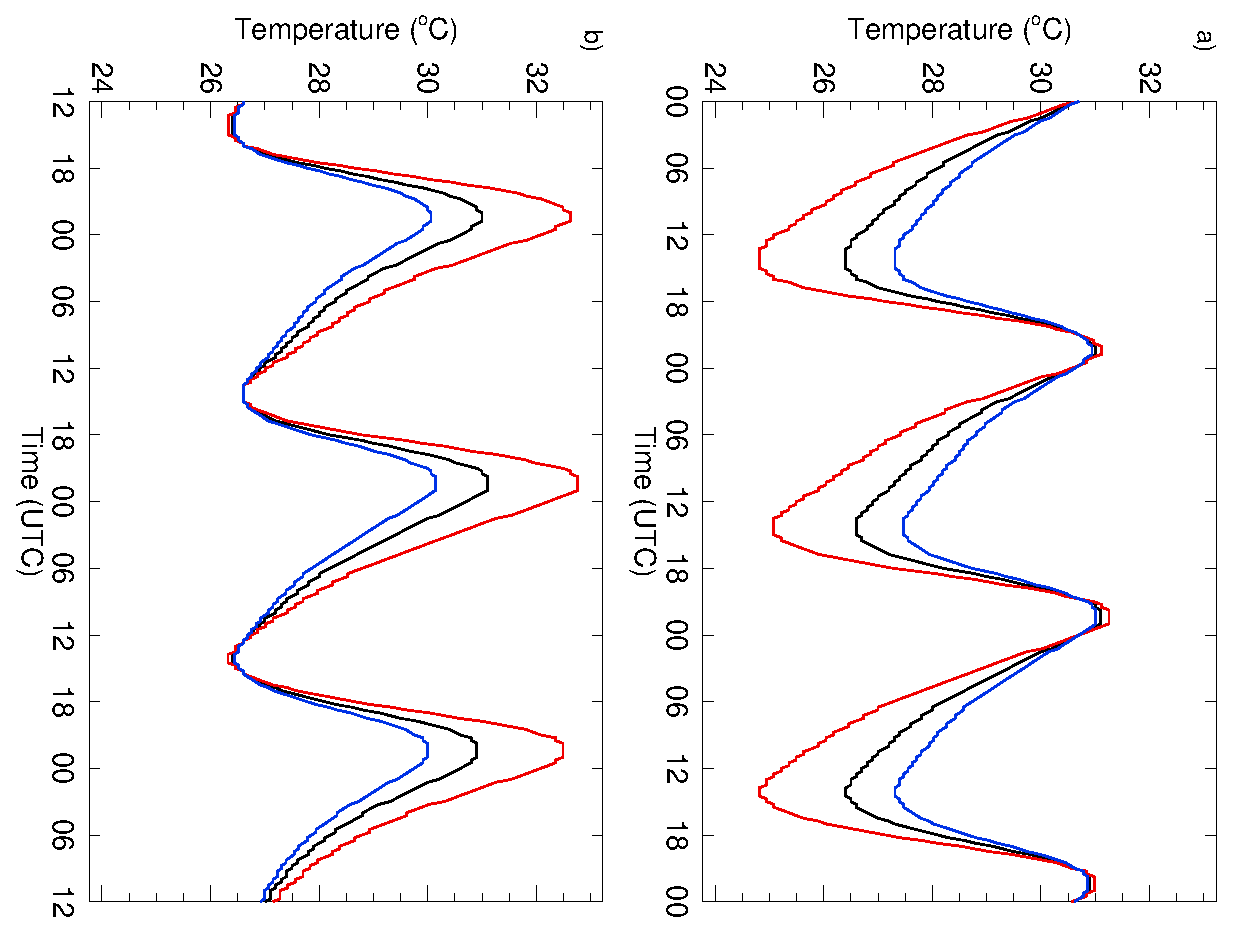
\includegraphics[angle=90, width=0.48\textwidth]{etacompfig9col}
\end{center}
\caption{
Slab soil model temperatures initialized by a) 0000 UTC
and b) 1200 UTC 5-cm soil temperature observations at Watonga on 20
July 2004.  Soil moisture errors of $+0.1$ m$^3$ m$^{-3}$ (blue) and
$-0.1$ m$^3$ m$^{-3}$ (red) yield temperatures that differ from
observed soil temperatures (black).
\label{etacompfig9}
}
\end{figure}
%%%%%%%%%%%%%%%%%%%%%%%%%%%%%%%%%%%%%%%%%%%%%%%%%%%%%%%%%%%%%%%%%%%%

\section{{\normalsize \hspace{-0.195in} {\textbf{
%%%Insert section heading below>>>>>>>>>>>>
CONCLUSIONS
%%%<<<<<<<<<<<<<<<<<<<<<<<<<<<<<<<<<<<<<<<<
}}}} \vspace{-1.6mm}
\label{etacomp_conc.sec}
This investigation compares soil temperature and soil moisture estimates from 40-km Eta analyses at several different model levels with observations from the Oklahoma Mesonet.  Eta analyses exhibit a systematic dry bias at all levels.  Consistent with the results of Marshall et al. (2003), soil temperatures in the most shallow soil layer tend to be too warm at 0000 UTC and too cool at 1200 UTC.  As previous studies have shown, soil temperature and soil moisture estimates strongly impact forecasts by numerical weather prediction models that implement sophisticated land surface parameterizations.  Problems with soil fields in Eta analyses, which provide initial conditions for a variety of research and operational modeling applications, may negatively impact the resulting model forecasts.  These existing biases suggest the strong need for an extensive network of soil observations, in addition to atmospheric surface observations, and the necessity for assimilating those observations into land surface initializations.
%END TEXT OF ARTICLE<<<<<<<<<<<

\begin{acknowledgments}
The authors wish to thank the Oklahoma Climatological Survey for providing Oklahoma Mesonet data.  Funding was provided under NSF grant ATM-0243720.
\end{acknowledgments}

%You could use BibTeX to create citations instead...

\begin{references}
{\footnotesize

\item Barnes, S. L., 1973: Mesoscale objective analysis using weighted time-series observations. NOAA Tech. Memo. ERL NSSL-62, National Severe Storms Laboratory, Norman, OK 73069, 60 pp. [NTIS COM-73-10781.]

\item Basara, J. B., and T. M. Crawford, 2000: Improved installation procedures for deep-layer soil moisture measurements. \textit{J. Atmos. Oceanic Technol.,} \textbf{17,} 879--884.

\item Beljaars, A. C. M., P. Viterbo, M. J. Miller, and A. Betts, 1996: The anomalous rainfall over the United States during July 1993: Sensitivity to land surface parameterization and soil moisture anomalies. \textit{Mon. Wea. Rev.,} \textbf{124,} 362--383.

\item Betts, A. K., J. H. Ball, A. C. M. Beljaars, M. J. Miller, and P. A. Viterbo, 1996: The land-surface-atmosphere interaction: A review based on observational and global modeling perspectives. \textit{J. Geophys. Res.,} \textbf{101(D3),} 7209--7226.

\item Bhumralkar, C. M., 1975: Numerical experiments on the computation of ground surface temperature in an atmospheric general circulation model. \textit{J. Appl. Meteor.,} \textbf{14,} 1246--1258.

\item Black, T. L., 1994: The new NMC mesoscale Eta model: Description and forecast examples. \textit{Wea. Forecasting,} \textbf{9,} 265--278.

\item Blackadar, A. K., 1976: Modeling the nocturnal boundary layer. Preprints, \textit{ Third Symp. on Atmospheric Turbulence, Diffusion and Air Quality,} Raleigh, NC, Amer. Meteor. Soc., 46--49.

\item Brennan, M. J., G. M. Lackmann, and S. E. Koch, 2003: An analysis of the impact of a split-front rainband on Appalachian cold-air damming. \textit{Wea. Forecasting,} \textbf{18,} 712--731.

\item Bright, D. R., and S. L. Mullen, 2002: The sensitivity of the numerical simulation of the southwest monsoon boundary layer to the choice of PBL turbulence parameterization in MM5. \textit{Wea. Forecasting,} \textbf{17,} 99--114.

\item Brock, F. V., K. C. Crawford, R. L. Elliot, G. W. Cuperus, S. J. Stadler, H. L. Johnson, and M. D. Eilts, 1995: The Oklahoma Mesonet: A technical overview. \textit{J. Atmos. Oceanic Technol.,} \textbf{12,} 5--19.

\item Brotzge, J. A., and K. C. Crawford, 2003: Examination of the surface energy budget: A comparison of eddy correlation and Bowen ratio measurement systems. \textit{J. Hydrometeor.,} \textbf{4,} 160--178.

\item Chen, F., and J. Dudhia, 2001: Coupling an advanced land surface-hydrology model with the Penn State--NCAR MM5 modeling system. Part I: Model implementation and sensitivity. \textit{Mon. Wea. Rev.,} \textbf{129,} 569--585.

\item ------, K. Mitchell, J. Schaake, Y. Xue, H.-L. Pan, V. Koren, Q. Y. Duan, M. Ek, and A. Betts, 1996: Modeling of land-surface evaporation by four schemes and comparison with FIFE observations. \textit{J. Geophys. Res.,} \textbf{101(D3),} 7251--7268.

\item Chen, Y., F. L. Ludwig, and R. L. Street, 2004: Stably stratified flows near a notched transverse ridge across the Salt Lake valley. \textit{J. Appl. Meteor.,} \textbf{43,} 1308--1328.

\item Clark, C., A., and R. W. Arritt, 1995: Numerical simulations of the effect of soil moisture and vegetation cover on the development of deep convection. \textit{J. Appl. Meteor.,} \textbf{34,} 2029--2045.

\item Colle, B. A., C. F. Mass, and D. Ovens, 2001: Evaluation of the timing and strength of MM5 and Eta surface trough passages over the eastern Pacific. \textit{Wea. Forecasting,} \textbf{16,} 553--572.

\item Cosby, B. J., G. M. Hornberger, R. B. Clapp, and T. R. Ginn, 1984: A statistical exploration of the relationships of soil moisture characteristics to the physical properties of soils. \textit{Water Resour. Res.,} \textbf{20,} 682--690.

\item Deardorff, J. W., 1978: Efficient prediction of ground surface temperature and moisture, with inclusion of a layer of vegetation. \textit{J. Geophys. Res.,} \textbf{83,} 1889--1903.

\item DiMego, G. J., and E. Rogers, cited 2005: Spring 2005 upgrade package for North American Mesoscale (NAM) decision brief. [Available online at\newline http://wwwt.emc.ncep.noaa.gov/mmb/Spring2005.NAMUpgrade.pdf.]

\item Dirmeyer, P. A., F. J. Zeng, A. Ducharne, J. C. Morrill, and R. D. Koster, 2000: The sensitivity of surface fluxes to soil water content in three land surface schemes. \textit{J. Hydrometeor.,} \textbf{1,} 121--134.

\item Ek, M. B., and A. A. M. Holtslag, 2004: Influence of soil moisture on boundary layer cloud development. \textit{J. Hydrometeor.,} \textbf{5,} 86--99.

\item Entekhabi, D., G. R. Asrar, A. K. Betts, K. J. Beven, R. L. Bras, C. J. Duffy, T. Dunne, R. D. Koster, D. P. Lettenmaier, D. B. McLaughlin, W. J. Shuttleworth, M. T. van Genuchten, M.-Y. Wei, and E. F. Wood, 1999: An agenda for land surface hydrology research and a call for the second international hydrological decade. \textit{Bull. Amer. Meteor. Soc.,} \textbf{80,} 2043--2058.

\item Entin, J. K., A. Robock, K. Y. Vinnikov, S. E. Hollinger, S. Liu, and A. Namkhai, 2000: Temporal and spatial scales of observed soil moisture variations in the extratropics. \textit{J. Geophys. Res.,} \textbf{105(D9),} 11 865--11 877.

\item Fennessy, M. J., and J. Shukla, 1999: Impact of initial soil wetness on seasonal atmospheric prediction. \textit{J. Climate,} \textbf{12,} 3167--3180.

\item Fulton, R. A., J. P. Breidenbach, D.-J. Seo, D. A. Miller, and T. O'Bannon, 1998: The WSR-88D Rainfall Algorithm. \textit{Wea. Forecasting,} \textbf{13,} 377--395.

\item Galewsky, J. and A. Sobel, 2005: Moist dynamics and orographic precipitation in northern and central California during the New Year's flood of 1997. \textit{Mon. Wea. Rev.,} \textbf{133,} 1594--1612.

\item Gannon, P. T., 1978: Influences of earth surface and cloud properties in the south Florida sea breeze. NOAA Tech. Rep. ERL402-NHELM2, 91 pp. [NTIS PB-297398.]

\item Gao, X., S. Sorooshian, and H. V. Gupta, 1996: A sensitivity analysis of the Biosphere-Atmosphere Transfer Scheme (BATS). \textit{J. Geophys. Res.,} \textbf{101 (D3),} 7279--7289.

\item Hart, K. A., W. J. Steenburgh, D. J. Onton, and A. J. Siffert, 2004: An evaluation of mesoscale-model-based model output statistics (MOS) during the 2002 Olympic and Paralympic Winter Games. \textit{Wea. Forecasting,} \textbf{19,} 200--218.

\item Hoadley, J. L., K. Westrick, S. A. Ferguson, S. L. Goodrick, L. Bradshaw, and P. Werth, 2004: The effect of model resolution in predicting meteorological parameters used in fire danger rating. \textit{J. Appl. Meteor.,} \textbf{43,} 1333--1347.

%\item Johansen, \O., 1975: Varmeledningsevne av Jordarter (Thermal conductivity of soils). Ph.D. thesis, University of Trondheim, 231 pp. [CRREL Draft Translation 637, 1977. Available from Defense Information Systems Agency, Defense Technical Information Center, 8725 John J. Kingman Road, Suite 0944, Fort Belvoir, VA 22060.]

\item Koren, V., J. Schaake, K. Mitchell, Q.-Y. Duan, F. Chen, and J. M. Baker, 1999: A parameterization of snowpack and frozen ground intended for NCEP weather and climate models. \textit{J. Geophys. Res.,} \textbf{104 (D16),} 19 569--19 585.

\item Koster, R. D., M. J. Suarez, P. Liu, U. Jambor, A. Berg, M. Kistler, R. Reichle, M. Rodell, and J. Famiglietti, 2004: Realistic initialization of land surface states: Impacts on subseasonal forecast skill. \textit{J. Hydrometeor.,} \textbf{5,} 1049--1063.

\item Leese, J., T. Jackson, A. Pitman, and P. Dirmeyer, 2001: GEWEX/BAHC International Workshop on Soil Moisture Monitoring, Analysis, and Prediction for Hydrometeorological and Hydroclimatological Applications. \textit{Bull. Amer. Meteor. Soc.,} \textbf{82,} 1423--1430. 

\item Lin, Y., K. E. Mitchell, E. Rogers, and G. J. DiMego, 2005: Using hourly and daily precipitation analyses to improve model water budget. Preprints, \textit{9th Symp. on Integrated Observing and Assimilation Systems for the Atmosphere, Oceans, and Land Surface,} San Diego, CA, Amer. Meteor. Soc., CD-ROM, 3.3.

\item Liu, Y., and R. Avissar, 1999a: A study of persistence in the land-atmosphere system using a general circulation model and observations. \textit{J. Climate,} \textbf{12,} 2139--2153.

\item ------, and ------, 1999b: A study of persistence in the land-atmosphere system with a fourth-order analytical model. \textit{J. Climate,} \textbf{12,} 2154--2168.

\item ------, D. Z. Ye, and J. J. Ji, 1993: Influence of soil moisture and vegetation on climate. Part II: Numerical experiments on persistence of short-term climatic anomalies. \textit{Sci. China,} \textbf{36B,} 102--109.

%\item Mahfouf, J.-F., 1991: Analysis of soil moisture from near-surface parameters: A
%feasibility study. \textit{J. Appl. Meteor.,} \textbf{30,} 1534--1547.

\item Mahrt, L., and H. L. Pan, 1984: A two-layer model of soil hydrology. \textit{Bound.-Layer Meteor.,} \textbf{29,} 1--20.

\item Marshall, C. H., K. C. Crawford, K. E. Mitchell, and D. J. Stensrud, 2003: The impact of the land surface physics in the operational NCEP Eta model on simulating the diurnal cycle: Evaluation and testing using Oklahoma Mesonet data. \textit{Wea. Forecasting,} \textbf{18,} 748--768.

\item McCumber, M. C., and R. A. Pielke, 1981: Simulation of the effects of surface fluxes of heat and moisture in a mesoscale numerical model. \textit{J. Geophys. Res.,} \textbf{86(C10),} 9929--9938.

\item Miller, D. A., and R. A. White, 1998: A conterminous United States multilayer soil characteristics dataset for regional climate and hydrology modeling. \textit{Earth Interactions,} \textbf{2,} 1--26.

\item Nelson, J. A., 1999: The Eta Data Assimilation System. WR Tech. Attachment 99-14, 6 pp. [Available from National Weather Service Western Region, P.O. Box 11188, Salt Lake City, UT 84147.]

\item Noilhan, J., and S. Planton, 1989: A simple parameterization of land-surface processes for meteorological models. \textit{Mon. Wea. Rev.,} \textbf{117,} 536--549.

\item Pan, H. L., and L. Mahrt, 1987: Interaction between soil hydrology and boundary-layer development. \textit{Bound.-Layer Meteor.,} \textbf{38,} 185--202.

\item Pielke, R. A., and X. Zeng, 1989: Influence on severe storm development of irrigated land. \textit{Natl. Wea. Dig.,} \textbf{14,} 16--17.

\item ------, G. E. Liston, J. L. Eastman, L. Lu., and M. Coughenour, 1999. \textit{J. Geophys. Res.,} \textbf{104(D16),} 19 463--19 479.

\item Rind, D., 1982: The influence of ground moisture conditions in North America on summer climate as modeled in the GISS GCM. \textit{Mon. Wea. Rev.,} \textbf{110,} 1487--1494.

\item Robock, A., K. Y. Vinnikov, G. Srinivasan, J. K. Entin, S. E. Hollinger, N. A. Speranskaya, S. Liu, and A. Namkhai, 2000: The global soil moisture data bank. \textit{Bull. Amer. Meteor. Soc.,} \textbf{81,} 1281--1299.

\item ------, L. Luo, E. F. Wood, F. Wen, K. E. Mitchell, P. R. Houser, J. C. Schaake, D. Lohmann, B. Cosgrove, J. Sheffield, Q. Duan, R. W. Higgins, R. T. Pinker, J. D. Tarpley, J. B. Basara, and K. C. Crawford, 2003: Evaluation of the North American Land Data Assimilation System over the southern Great Plains during the warm season. \textit{J. Geophys. Res.,} \textbf{108,} 8846, doi:10.1029/2002JD003245.

\item Rodell, M., P. R. Houser, A. A. Berg, and J. S. Famiglietti, 2005: Evaluation of 10 methods for initializing a land surface model. \textit{J. Hydrometeor.,} \textbf{6,} 146--155.

\item Rogers, E., T. L. Black, D. G. Deaven, G. J. DiMego, Q. Zhao, M. Baldwin, N. W. Junker, and Y. Lin, 1996: Changes to the operational "early" Eta analysis/forecast system at the National Centers for Environmental Prediction. \textit{Wea. Forecasting,} \textbf{11,} 391--413.

%Using \vspace between references on the last page is a simple way to balance
%the columns within an environment where something like the package balance.sty
%won't do the trick.
\vspace{0.235mm}

\item Rowntree, P. R., and J. A. Bolton, 1983: Simulation of the atmospheric response to soil moisture anomalies over Europe. \textit{Quart. J. Roy. Meteor. Soc.,} \textbf{109,} 501--526.

\vspace{0.235mm}

\item Schlatter, T. W., 1975: Some experiments with a multivariate statistical objective analysis scheme. \textit{Mon Wea. Rev.,} \textbf{103,} 246--257.

\vspace{0.235mm}

\item Sellers, P. J., Y. Mintz., Y. C., Sud, and A. Dalcher, 1986: A simple biosphere model (SiB) for use within general circulation models. \textit{J. Atmos. Sci.,} \textbf{43,} 505--531. 

\vspace{0.235mm}

\item Seuffert, G., H. Walker, P. Viterbo, M. Drusch, and J.-F. Mahfouf, 2004: The usage of screen-level parameters and microwave brightness temperature for soil moisture analysis. \textit{J. Hydrometeor.,} \textbf{5,} 516--531.

\vspace{0.235mm}

\item Shafer, M. A., C. A. Fiebrich, D. S. Arndt, S. E. Fredrickson, and T. W. Hughes, 2000: Quality assurance procedures in the Oklahoma Mesonetwork. \textit{J. Atmos. Sci.,} \textbf{17,} 474--494.

\vspace{0.235mm}

\item Smith, C. B., M. N. Lakhtakia, W. J. Capehart, and T. N. Carlson, 1994: Initialization of soil-water content in regional-scale atmospheric prediction models. \textit{Bull. Amer. Meteor. Soc.,} \textbf{74,} 585--593.

\vspace{0.235mm}

\item Stensrud, D. J., and S. J. Weiss, 2002: Mesoscale model ensemble forecasts of the 3 May 1999 tornado outbreak. \textit{Wea. Forecasting,} \textbf{17,} 526--543.

\vspace{0.235mm}

\item Stensrud, D. J., N. Yussouf, M. E. Baldwin, J. T. McQueen, J. Du, B. Zhou, B. Ferrier, G. Manikin, F. M. Ralph, J. M. Wilczak, A. B. White, I. Djlalova, J.-W. Bao, R. J. Zamora, S. G. Benjamin, P. A. Miller, T. L. Smith, T. Smirnova, and M. F. Barth, 2005: The New England high-resolution temperature program (NEHRTP). \textit{Bull. Amer. Meteor. Soc.,} submitted.

\vspace{0.235mm}

\item Troen, I., and L. Mahrt, 1986: A simple model of the boundary layer: Sensitivity to surface evaporation. \textit{Bound.-Layer Meteor.,} \textbf{37,} 129--148.

\vspace{0.235mm}

\item Twine, T. E., C. J. Kucharik, and J. A. Foley, 2004: Effects of land cover change on the energy and water balance of the Mississippi River basin. \textit{J. Hydrometeor.,} \textbf{5,} 640--655.

\vspace{0.235mm}

\item Vinnikov, K. Y., and I. B. Yeserkepova, 1991: Soil moisture: Empirical data and model results. \textit{J. Climate,} \textbf{4,} 66--79.

\vspace{0.235mm}

\item ------, A. Robock, N. A. Speranskaya, and C. A. Schlosser, 1996: Scales of temporal and spatial variability of midlatitude soil moisture. \textit{J. Geophys. Res.,} \textbf{101(D3),} 7163--7174.

\newpage

\item Viterbo, P., and A. C. M. Beljaars, 1995: An improved land surface parameterization scheme in the ECMWF model and its validation. \textit{J. Climate,} \textbf{8,} 2716--2748.

\item ------, and A. K. Betts, 1999: Impact of the ECMWF reanalysis soil water on forecasts of the July 1993 Mississippi flood. \textit{J. Geophys. Res.,} \textbf{104(D16),} 19 361--19 366.

\item Walker, J. M., and P. R. Rowntree, 1977: The effect of soil moisture on circulation and rainfall in a tropical model. \textit{Quart. J. Roy. Meteor. Soc.,} \textbf{103,} 29--46.

\item Walsh, J. E., W. H. Jasperson, and B. Ross, 1985: Influence of snow cover and soil moisture on monthly air temperature. \textit{Mon. Wea. Rev.,} \textbf{113,} 756--768.

\item Wei, M.-Y., Ed., 1995: Soil Moisture: Report of a Workshop Held in Tiburon, California, 25--27 January 1994. NASA Conference Publication 3319, 80 pp.

\item Westrick, K. J., P. Storck, and C. F. Mass, 2002: Description and evaluation of a hydrometeorological forecast system for mountainous watersheds. \textit{Wea. Forecasting,} \textbf{17,} 250--262.

\item Wilks, D. S., 1995: \textit{Statistical Methods in the Atmospheric Sciences.} International Geophysics Series, Vol. 59, Academic Press, 464 pp.

\item Xu, Q., and B. Zhou, 2003: Retrieving soil water contents from soil temperature measurements by using linear regression. \textit{Adv. Atmos. Sci.,} \textbf{20,} 849--858.

\item Yan, H., and R. A. Anthes, 1988: The effect of variations in surface moisture on mesoscale circulations. \textit{Mon. Wea. Rev.,} \textbf{116,} 192--208.

\item Yeh, T.-C., R. T. Wetherald, and S. Manabe, 1984: The effect of soil moisture on the short-term climate and hydrology change -- A numerical experiment. \textit{Mon. Wea. Rev.,} \textbf{112,} 474--490.

\item Zamora, R. J., E. G. Dutton, M. Trainer, S. A. McKeen, J. M. Wilczak, and Y.-T. Hou, 2005: The accuracy of solar irradiance calculations used in mesoscale numerical weather prediction. \textit{Mon. Wea. Rev.,} \textbf{133,} 783--792.

\item Zehnder, J. A., 2002: Simple modifications to improve fifth-generation Pennsylvania State University--National Center for Atmospheric Research  Mesoscale Model performance for the Phoenix, Arizona, metropolitan area. \textit{J. Appl. Meteor.,} \textbf{41,} 971--979.

\item Zhong, S., H.-J. In, X. Bian, J. Charney, W. Heilman, and B. Potter, 2005: Evaluation of real-time high-resolution MM5 predictions over the Great Lakes region. \textit{Wea. Forecasting,} \textbf{20,} 63--81.

\item Zobler, L., 1986: A world soil file for global climate modeling. NASA Tech. Memo. 87802, 32 pp.

}	%End footnotesize
\end{references}


\end{document}
